% ============================================================
%  Murphy-Health — One-Pager
%  Track 01 · Insilico Medicine Longevity Hackathon
%  Compile:  pdflatex one_pager.tex   (run twice for equal-height boxes)
% ============================================================
\documentclass[10pt,a4paper]{article}

% ---------- packages ----------
\usepackage[margin=0.4in,top=0.35in,bottom=0.25in]{geometry}
\usepackage[T1]{fontenc}
\usepackage{lmodern}
\usepackage{amsmath}
\usepackage{amssymb}
\usepackage{xcolor}
\usepackage{graphicx}
\usepackage[skins]{tcolorbox}
\usepackage{enumitem}
\usepackage{tikz}
\usepackage{hyperref}
\usepackage{titlesec}
\usepackage{fontawesome5}

% ---------- bamboo palette (matches CLI theme) ----------
\definecolor{bamboodark}{RGB}{45,80,25}
\definecolor{bamboomid}{RGB}{100,145,55}
\definecolor{bamboolight}{RGB}{195,225,100}
\definecolor{bambooshoot}{RGB}{165,200,85}
\definecolor{cardbg}{RGB}{249,251,239}
\definecolor{phgray}{RGB}{140,140,140}

\setlist[itemize]{leftmargin=11pt, topsep=2pt, itemsep=1pt, parsep=0pt}

\pagestyle{empty}
\setlength{\parindent}{0pt}

\titleformat{\section}{\large\bfseries\color{bamboodark}}{}{0pt}{}
\titlespacing*{\section}{0pt}{8pt}{2pt}

% ---------- solution card style ----------
\tcbset{
  solutionbox/.style={
    colback=cardbg,
    colframe=bamboomid,
    boxrule=0.6pt,
    arc=2.5pt,
    left=5pt, right=5pt, top=2pt, bottom=3pt,
    fonttitle=\small\bfseries,
    coltitle=bamboodark,
    colbacktitle=cardbg,
    equal height group=sol
  },
  pipebox/.style={
    colback=cardbg,
    colframe=bamboomid,
    boxrule=0.5pt,
    arc=2pt,
    left=5pt, right=5pt, top=3pt, bottom=3pt,
    fonttitle=\footnotesize\bfseries,
    coltitle=bamboodark,
    colbacktitle=cardbg,
    title=\hbox{}
  }
}

% ---------- placeholder boxes ----------
\newcommand{\imgph}[3]{%
  \begin{tikzpicture}
    \draw[bamboomid, dashed, line width=0.5pt, rounded corners=2pt]
      (0,0) rectangle (#1, #2);
    \node[align=center, text width=#1, font=\footnotesize\itshape\color{phgray}]
      at (#1/2, #2/2) {\faImage[regular]\\[2pt]#3};
  \end{tikzpicture}%
}

% ---------- rounded-corner 16:9 image (with bamboo hairline) ----------
% #1 = TeX length (e.g. \linewidth, 4.85cm); #2 = image path
\newlength{\rcw}
\newlength{\rch}
\newcommand{\rcimg}[2]{%
  \setlength{\rcw}{#1}%
  \setlength{\rch}{0.5625\rcw}%
  \begin{tikzpicture}
    \begin{scope}
      \path[clip, rounded corners=3pt] (0,0) rectangle (\rcw, \rch);
      \node[anchor=south west, inner sep=0] at (0,0)
        {\includegraphics[width=\rcw]{#2}};
    \end{scope}
    \draw[bamboomid, line width=0.5pt, rounded corners=3pt]
      (0,0) rectangle (\rcw, \rch);
  \end{tikzpicture}%
}

% ---------- formula card: same 16:9 footprint as \rcimg, no frame ----------
% #1 = TeX length; #2 = content (display math + optional gloss)
\newcommand{\formulabox}[2]{%
  \setlength{\rcw}{#1}%
  \setlength{\rch}{0.5625\rcw}%
  \begin{tikzpicture}
    \path (0,0) rectangle (\rcw, \rch);
    \node[align=center, text width=\dimexpr \rcw - 3mm\relax, inner sep=0]
      at (0.5\rcw, 0.5\rch) {#2};
  \end{tikzpicture}%
}

% ---------- square headshot (already pre-cropped) ----------
\newcommand{\headshot}[2][1.05cm]{%
  \begin{tikzpicture}
    \node[inner sep=1pt, draw=bamboomid, line width=0.5pt,
          dashed, rounded corners=2pt] (h)
      {\includegraphics[width=#1, height=#1]{headshots_sq/#2}};
  \end{tikzpicture}%
}

% ---------- pipeline item: bold tool + light gloss ----------
\newcommand{\tool}[2]{%
  \textbf{\color{bamboodark}#1}\,{\color{phgray}\tiny\,#2}%
}

\begin{document}

% ============================================================
%  HEADER
% ============================================================
\begin{center}
{\Huge\bfseries\color{bamboodark} Murphy-Health}\\[2pt]
{\small\color{bamboomid}\itshape An Estimathon-Style Iterative Benchmark for Longevity LLMs}\\[1pt]
{\footnotesize Caltech Longevity Hackathon \textbullet{} Track 01 \textbullet{} LongevityLLM Benchmarking \textbullet{} May 23, 2026}
\end{center}

\vspace{-4pt}
{\color{bamboomid}\hrule height 0.8pt}
\vspace{3pt}

% ============================================================
%  THE PROBLEM
% ============================================================
\section*{The Problem}
\noindent
\begin{minipage}[t]{0.62\textwidth}
\vspace{0pt}
Current longevity LLM benchmarks (incl.\ \emph{LongeBench}) have three blind spots that let a model look smart without actually \emph{being calibrated}:
\begin{itemize}
  \item \textbf{Limited topic coverage.} RNA-level aging biology --- enzymes, disease/hallmark associations, pathway regulation --- is sparsely represented relative to its weight in real aging research.
  \item \textbf{Detection only, no estimation.} Tasks are dominated by binary / multi-class classification. Few measure a model's ability to put a \emph{calibrated number} on an aging biomarker.
  \item \textbf{One-shot, no self-correction.} Existing benchmarks score a single final answer. None test whether a model can \emph{iterate} under partial feedback or \emph{recognize its own mistakes} when its guess is rejected.
\end{itemize}
Real biology demands calibrated uncertainty \emph{and} the ability to refine --- right answers for the wrong reasons should not pass.
\end{minipage}\hfill
\begin{minipage}[t]{0.35\textwidth}
\vspace{0pt}
\centering
\imgph{5.5cm}{3.3cm}{Figure placeholder\\RNA $\leftrightarrow$ aging regulation\\(literature reference)}
\\[2pt]
{\scriptsize\color{phgray}\itshape Anchors the scientific basis of our new question bank.}
\end{minipage}

% ============================================================
%  THE SOLUTION
% ============================================================
\section*{The Solution}
\vspace{3pt}

\noindent
\begin{minipage}[t]{0.325\textwidth}
\centering
\rcimg{\linewidth}{pictures_169/HF.jpg}\par
\vspace{3pt}
\begin{tcolorbox}[solutionbox, title={\faDatabase~~1. RNA Question Bank}]
\raggedright\scriptsize
\textbf{What we built.} Two curated RNA-aging question banks published openly on HuggingFace: \texttt{carolw/EP04} (enzyme--disease pairs from aging-phenotype enzymes) and \texttt{sarahliu/rna-eb0x} (RNA expression, hallmark and pathway regulation).\\[2pt]
\textbf{How we built it.} Seeded from primary literature, auto-labeled with abstract retrieval, hand-verified, then \emph{adversarially filtered} against SotA LLMs --- only questions where strong models disagree or err survive.\\[2pt]
\textbf{Why it matters.} Plugs the RNA / early-detection gap in LongeBench, and is \emph{ungated}: one CLI flag pulls it.
\end{tcolorbox}
\end{minipage}\hfill
%
\begin{minipage}[t]{0.325\textwidth}
\centering
\formulabox{\linewidth}{%
  {\small%
    $\displaystyle S = \Bigl(10 + \!\!\sum_{i\in\mathcal{G}}\! \bigl\lfloor \tfrac{u_i}{l_i} \bigr\rfloor \Bigr) \cdot 2^{\,N-|\mathcal{G}|}$%
  }\\[4pt]
  {\tiny\color{phgray}\itshape $[l_i,u_i]$ = last interval on problem $i$;\\
   $\mathcal{G}$ = set of GOOD final answers;\,lower $S$ wins.}%
}\par
\vspace{3pt}
\begin{tcolorbox}[solutionbox, title={\faChartLine~~2. The Algo --- Estimathon}]
\raggedright\scriptsize
\textbf{Mechanic.} Each problem gets an interval $[l_i,u_i]$. The model sees \emph{only} GOOD / BAD --- no directional hint. A shared budget of $\lfloor \tfrac{18}{13}N \rfloor$ slips is split across all $N$ problems; cap 3 slips/problem.\\[2pt]
\textbf{Why this works.} Width factor $\lfloor u/l\rfloor$ punishes hedged ``[1,\,100]'' answers; the $2^{N-|\mathcal{G}|}$ term punishes leaving problems empty. Refinement is a \emph{voluntary bet}: random guessing wins 50\%, so beating 50\% is genuine biological reasoning, not bracket-search.
\end{tcolorbox}
\end{minipage}\hfill
%
\begin{minipage}[t]{0.325\textwidth}
\centering
\rcimg{\linewidth}{pictures_169/convo.jpg}\par
\vspace{3pt}
\begin{tcolorbox}[solutionbox, title={\faTerminal~~3. The Program --- CLI}]
\raggedright\scriptsize
\textbf{Install.} \texttt{pip install murthy-bench}; first run launches an API-key + HF-token wizard.\\[2pt]
\textbf{One command, any model, any data.} \texttt{murthy run --model X --provider Y --tasks Z} works for Anthropic, OpenAI, the Insilico L-LLM endpoint, or any HF inference URL --- mix-and-match.\\[2pt]
\textbf{Interactive chat.} \texttt{/test}, \texttt{/batch}, \texttt{/model}, \texttt{/explore} slash commands with autocomplete; live progress bar, per-slip $\langle$think$\rangle$ trace capture, JSONL results for downstream analysis.
\end{tcolorbox}
\end{minipage}

% ============================================================
%  PIPELINE  (replaces tech stack)
% ============================================================
\section*{Pipeline}
\vspace{-1pt}
\begin{center}
\begin{tikzpicture}[
  font=\scriptsize,
  pipe/.style={draw=bamboomid, line width=0.5pt, fill=cardbg,
               rounded corners=3pt, text width=3.55cm,
               minimum height=1.45cm, align=center, inner sep=4pt,
               anchor=north west},
  band/.style={draw=bamboomid, line width=0.4pt, fill=cardbg,
               rounded corners=3pt, align=center, inner sep=4pt},
  arrow/.style={->, >=stealth, draw=bamboomid, line width=0.9pt}
]
\node (data)   at (0,0)    [pipe] {\textbf{\color{bamboodark}\faDatabase\,\,DATA}\\[1pt]
  \tiny LongeBench (HF gated)\\
  \texttt{carolw/EP04}\\
  \texttt{sarahliu/rna-eb0x}\\
  JSONL schema};
\node (engine) at (4.05,0) [pipe] {\textbf{\color{bamboodark}\faCogs\,\,ENGINE}\\[1pt]
  \tiny Estimathon session\\
  Iterative slip + score\\
  Refinement-accuracy\\
  One-shot (8-thread)};
\node (model)  at (8.1,0)  [pipe] {\textbf{\color{bamboodark}\faRobot\,\,MODELS}\\[1pt]
  \tiny Anthropic SDK\\
  OpenAI SDK\\
  HF Hub Registry (300+)\\
  Insilico L-LLM endpoint};
\node (out)    at (12.15,0)[pipe] {\textbf{\color{bamboodark}\faFileCode\,\,OUTPUT}\\[1pt]
  \tiny \texttt{results.jsonl}\\
  Live progress bar\\
  \texttt{<think>} traces\\
  Per-format breakdown};
\draw[arrow] (data.east)   -- (engine.west);
\draw[arrow] (engine.east) -- (model.west);
\draw[arrow] (model.east)  -- (out.west);
\node (band) [band, text width=15.55cm, minimum height=0.45cm, anchor=north west]
  at (0, -1.65) {%
  \tiny \textbf{\color{bamboodark}CLI surface:} Typer \textbullet\ Rich \textbullet\ prompt\_toolkit \textbullet\ slash autocomplete \textbullet\ live progress
  \quad\textbar\quad
  \textbf{\color{bamboodark}Distribution:} \texttt{pip install murthy-bench} \textbullet\ GitHub Actions + OIDC trusted publish on \texttt{v*} tag};
\draw[bamboomid, line width=0.4pt, dashed]
  (band.north -| data.center)   -- (data.south);
\draw[bamboomid, line width=0.4pt, dashed]
  (band.north -| engine.center) -- (engine.south);
\draw[bamboomid, line width=0.4pt, dashed]
  (band.north -| model.center)  -- (model.south);
\draw[bamboomid, line width=0.4pt, dashed]
  (band.north -| out.center)    -- (out.south);
\end{tikzpicture}
\end{center}

% ============================================================
%  TEAM
% ============================================================
\section*{Team}
\vspace{-1pt}
\noindent
\begin{minipage}[t]{0.188\textwidth}
\centering
\headshot{Michael.jpg}\\[2pt]
\textbf{\scriptsize Yiqi (Michael) Yao}\\[1pt]
{\tiny\color{phgray}
Harvey Mudd College, '29\\
Joint CS \& Mathematics\\
\href{mailto:miyao@g.hmc.edu}{miyao@g.hmc.edu}}\\[2pt]
{\scriptsize\itshape\color{bamboodark}
CLI architecture, scoring engine, packaging \& test pipeline}
\end{minipage}\hfill
\begin{minipage}[t]{0.188\textwidth}
\centering
\headshot{Olivia.jpg}\\[2pt]
\textbf{\scriptsize Yan (Olivia) Yan}\\[1pt]
{\tiny\color{phgray}
Harvey Mudd College, '29\\
Math \& Computational Biology\\
\href{mailto:oyan@g.hmc.edu}{oyan@g.hmc.edu}}\\[2pt]
{\scriptsize\itshape\color{bamboodark}
Insilico L-LLM integration, LongeBench wiring, open-source model curation for benchmark testing, head chef~\faUtensils}
\end{minipage}\hfill
\begin{minipage}[t]{0.188\textwidth}
\centering
\headshot{Sarah.jpg}\\[2pt]
\textbf{\scriptsize Yuhui (Sarah) Liu}\\[1pt]
{\tiny\color{phgray}
Harvey Mudd College, '28\\
Joint Chemistry \& Biology\\
\href{mailto:saraliu@g.hmc.edu}{saraliu@g.hmc.edu}}\\[2pt]
{\scriptsize\itshape\color{bamboodark}
RNA research lead --- disease/hallmark, pathway regulation; Q-bank curation \& SotA testing}
\end{minipage}\hfill
\begin{minipage}[t]{0.188\textwidth}
\centering
\headshot{Carol.jpg}\\[2pt]
\textbf{\scriptsize Xiaokuan (Carol) Wang}\\[1pt]
{\tiny\color{phgray}
Harvey Mudd College, '29\\
Math \& Computational Biology\\
\href{mailto:carowang@g.hmc.edu}{carowang@g.hmc.edu}}\\[2pt]
{\scriptsize\itshape\color{bamboodark}
RNA research --- aging-phenotype enzymes; Q-bank curation \& SotA testing}
\end{minipage}\hfill
\begin{minipage}[t]{0.188\textwidth}
\centering
\headshot{Chun-Yu.jpg}\\[2pt]
\textbf{\scriptsize Chun-Yu (Alex) Chen}\\[1pt]
{\tiny\color{phgray}
Claremont McKenna College, '29\\
Math \& Computational Biology\\
\href{mailto:cchen29@cmc.edu}{cchen29@cmc.edu}}\\[2pt]
{\scriptsize\itshape\color{bamboodark}
Project architecture, scoring-function ideation, documentation, diversity debugging, two-day round-trip driver~\faCar}
\end{minipage}

% ============================================================
%  FOOTER
% ============================================================
\vfill
{\color{bamboomid}\hrule height 0.4pt}
\vspace{3pt}
\begin{center}
\footnotesize
\textcolor{bamboodark}{\faGithub}~\href{https://github.com/OhhMoo/Murphy-Health}{github.com/OhhMoo/Murphy-Health}
\quad\textcolor{bamboomid}{\textbullet}\quad
\textcolor{bamboodark}{\faDatabase}~\href{https://huggingface.co/datasets/carolw/EP04train_and_set/tree/main/my_folder}{carolw/EP04train\_and\_set}
\quad\textcolor{bamboomid}{\textbullet}\quad
\textcolor{bamboodark}{\faDatabase}~\href{https://huggingface.co/datasets/sarahliu/rna-eb0x/tree/main}{sarahliu/rna-eb0x}
\quad\textcolor{bamboomid}{\textbullet}\quad
\textcolor{bamboodark}{\faDownload}~\texttt{pip install murthy-bench}
\end{center}

\end{document}
